\section{Discussion and Related Work}

\begin{frame}{Discussion and Related Work}
\end{frame}

\begin{frame}{Limitations of Evaluation (Synthetic Data)}

  \begin{block}{Alphabet size}
    \begin{itemize}
      \item Binary alphabets only; state of the art in GI evaluations
      \item In contrast, more than 30 events is commonly observed in behavior models
    \end{itemize}
  \end{block}

  \begin{block}{State machines}
    \begin{itemize}
      \item No variance of state degree, as a consequence of binary alphabet 
      \item States with high in-/out degrees are commonly observed in behavior model 
            (capturing system \emph{idle}, \emph{halt}, \emph{immediate response})
    \end{itemize}
  \end{block}

  \begin{block}{Samples}
    \begin{itemize}
      \item Randomly generated from uniform distribution of strings
      \item Not representative of what should be generated "from the machine", especially 
            on large alphabets
    \end{itemize}
  \end{block}

\end{frame}

\begin{frame}{The Stamina Competition}

  \begin{center}
    
\includegraphics[width=12cm]{images/stamina.jpg}
  \end{center}

  \begin{itemize}
    \item Online Regular Induction Contest
    \item Extends former competitions, especially Abbadingo
    \item Focusses on the complexity of the learning with respect to the alphabet size
    \item Adapted generation protocol for state machines and samples
    \item Cross-fertilization between the machine learning and software engineering communities
  \end{itemize}

\end{frame}

\begin{frame}{Stamina: Principle}

  \begin{columns}
    \column{.4\textwidth}
	  \begin{itemize}
	    \item 100 induction problems (20 cells, 5 problems each)
	    \item Two difficulty dimensions: alphabet size vs. sparsity of learning sample
	  \end{itemize}
    \column{.6\textwidth}
	  \begin{center}
	    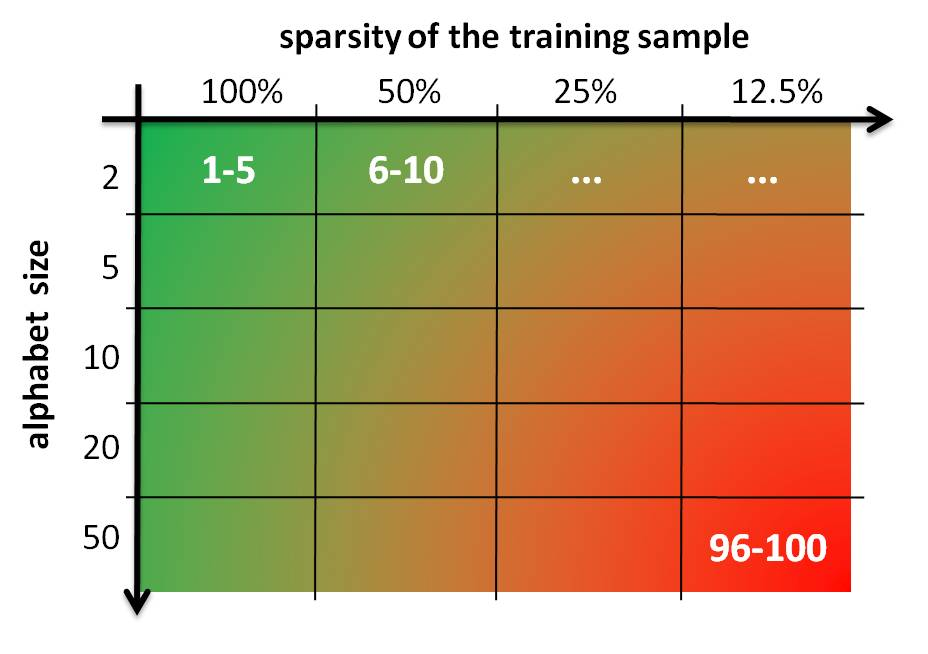
\includegraphics[width=6cm]{images/stamina_grid.jpg}
	  \end{center}
  \end{columns}

  \begin{block}{Solving a problem}
    \begin{itemize}
      \item Download learning (labeled) and test (unlabeled) samples
      \item Learn a model (typically a DFA)
      \item Label the test sample using learned model
      \item Submit labeling on the competition server
    \end{itemize}
  \end{block}


\end{frame}

\begin{frame}{Scientific setup: State machines}

  \begin{block}{Approach}
    \begin{itemize}
      \item Review of SE litterature to identify representative features of behavior models
      \item Tuning of the Forest-fire algorithm to mimic these features
    \end{itemize}
  \end{block}

  \begin{block}{Main features}
    \begin{itemize}
      \item Approximately 50 states (to avoid adding a third difficulty dimension to the competition)
      \item Alphabet sizes ranging from 2 to 50 letters
      \item Equal proportion of accepting vs. rejecting states
      \item Large variance of degree distribution, to mimic behavior models
    \end{itemize}
  \end{block}

\end{frame}

\begin{frame}{Scientific setup: Samples}

  \begin{block}{Approach}
    \begin{itemize}
      \item Generated by the target machine, using a random walk algorithm
      \item Negative strings obtained by randomly perturbing positive ones
      \begin{itemize}
        \item three kinds of edit: substitution, insertion and deletion of letters
      \end{itemize}
      \item Tuned to ensure good induction results using Blue-Fringe on the simplest 
            problems
    \end{itemize}
  \end{block}

  \begin{block}{Main features}
    \begin{itemize}
      \item Learning and test samples do not overlap
      \item Learning samples may contain duplicates, as a consequence of the random walk generation
      \item Length distribution of strings centered on $5 + depth(automaton)$
    \end{itemize}
  \end{block}

\end{frame}

\begin{frame}{Scientific setup: Submission and Scoring}

  \begin{block}{Submission}
    \begin{itemize}
      \item Solutions submitted as binary strings labelling the test sample
      \item Binary feedback (problem broken or not broken), to avoid hill-climbing
    \end{itemize}
  \end{block}

  \begin{block}{Scoring}
    \begin{itemize}
      \item Balanced Classification Rate to place equal emphasis on accuracy in terms of positive 
            and negative strings
      \item Problem broken if BCR score >= 0.99
      \item A cell is broken if all problems it contains are broken
    \end{itemize}
  \end{block}

\end{frame}

\begin{frame}{Balanced Classification Rate (BCR)}

  \begin{block}{Sensitivity \& Specificity}
    Sensitivity (resp. Specificity): \emph{how well does the learner accept (resp. reject)
    positive strings (resp. negative strings)?}
    \begin{center}
    \begin{math}
      Sensitivity=\frac{|TP|}{|TP \cup FN|},
      Specificity=\frac{|TN|}{|TN \cup FP|}
    \end{math}
    \end{center}
    Where $TP$, $FP$, $TN$ and $FN$ stand for True/False Positive/Negative
  \end{block}

  \begin{block}{Harmonic Balanced Classification Rate}
    \begin{center}$HBCR=\frac{2*Sensitivity*Specificity}{Sensitivity + Specificity}$\end{center}
    \emph{Harmonic} BCR prefered over arithmetic: favors a good balance between sensitivity 
    and specificity
  \end{block}

\end{frame}

\begin{frame}{Scientific setup: Baseline}

  Problem grid empirically ajusted 
	\begin{itemize}
	\item To ensure good induction results using Blue-Fringe on the simplest problems
	\item Without breaking the cell
	\end{itemize}

  \begin{center}
    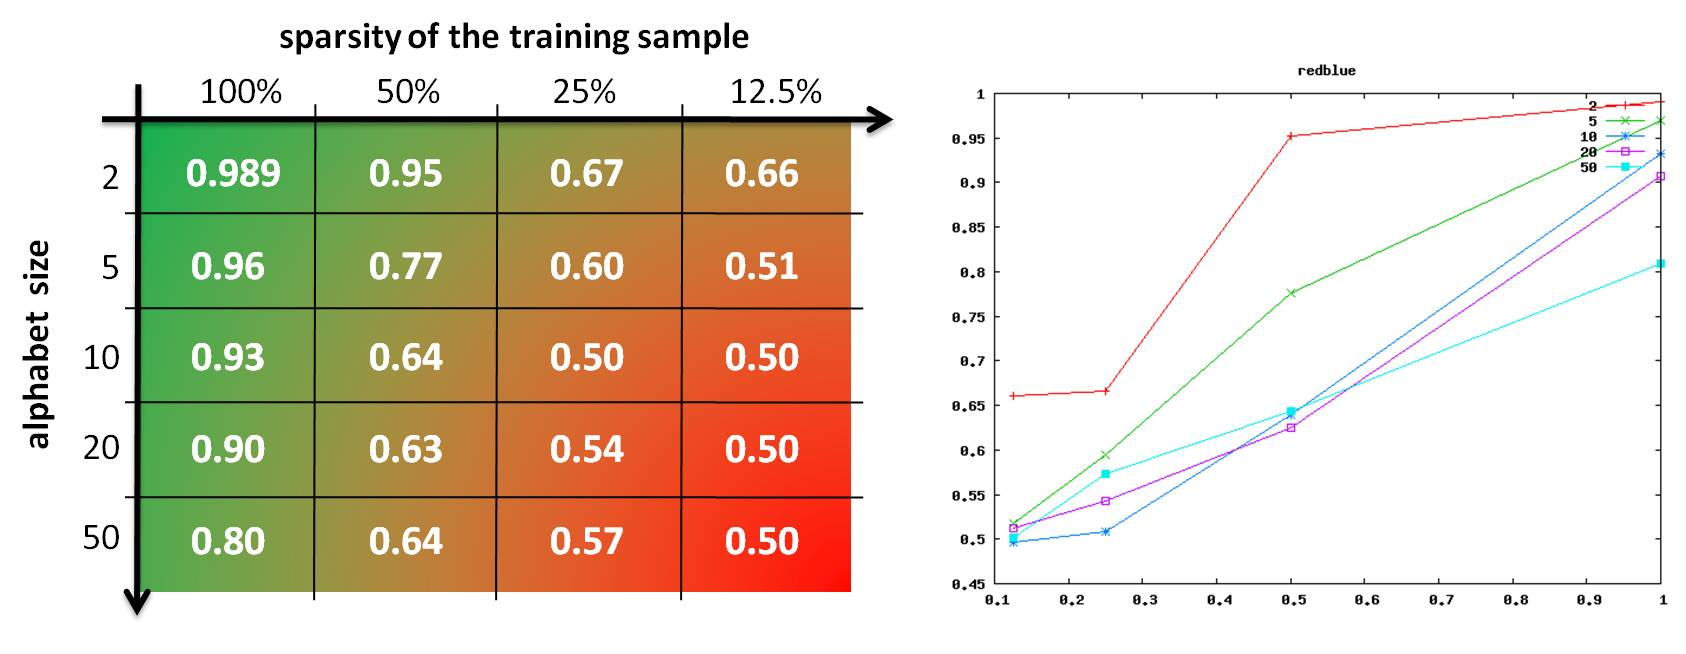
\includegraphics[width=11cm]{images/stamina_baseline.jpg}
  \end{center}

\end{frame}

\begin{frame}{Baseline: lessons learned}

  \begin{itemize}
    \item RPNI and BlueFringe still converge, even on largest alphabets
	  \begin{itemize}
	    \item Theoretically expected, big samples needed in practice
	  \end{itemize}
    \item Size of the alphabet "hurts" convergence in practice
	  \begin{itemize}
	    \item Confirms experimentally what we expected theoretically 
	    \item Supports launching of Stamina
	  \end{itemize}
  \end{itemize}

  \begin{center}
    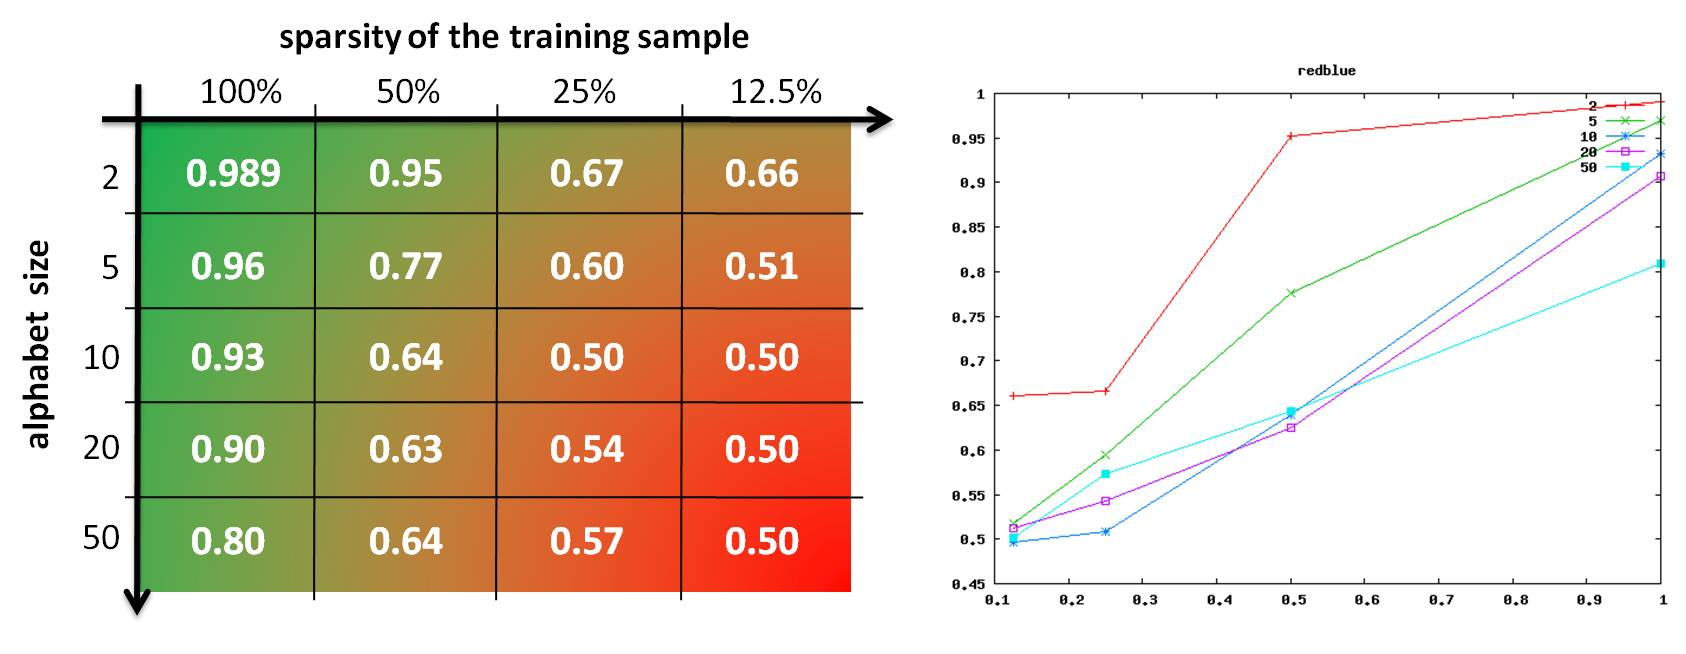
\includegraphics[width=11cm]{images/stamina_baseline.jpg}
  \end{center}

\end{frame}

\begin{frame}{Some competition data}
  \begin{itemize}
    \item Ran between march and december 2010
    \item 1856 submissions made by 11 challengers, 
    \item 65 winning submissions leading to 42 problems broken
    \item 6 cells completely broken, by 2 challengers (Equipo \& DFASAT)
  \end{itemize}

  \begin{center}
    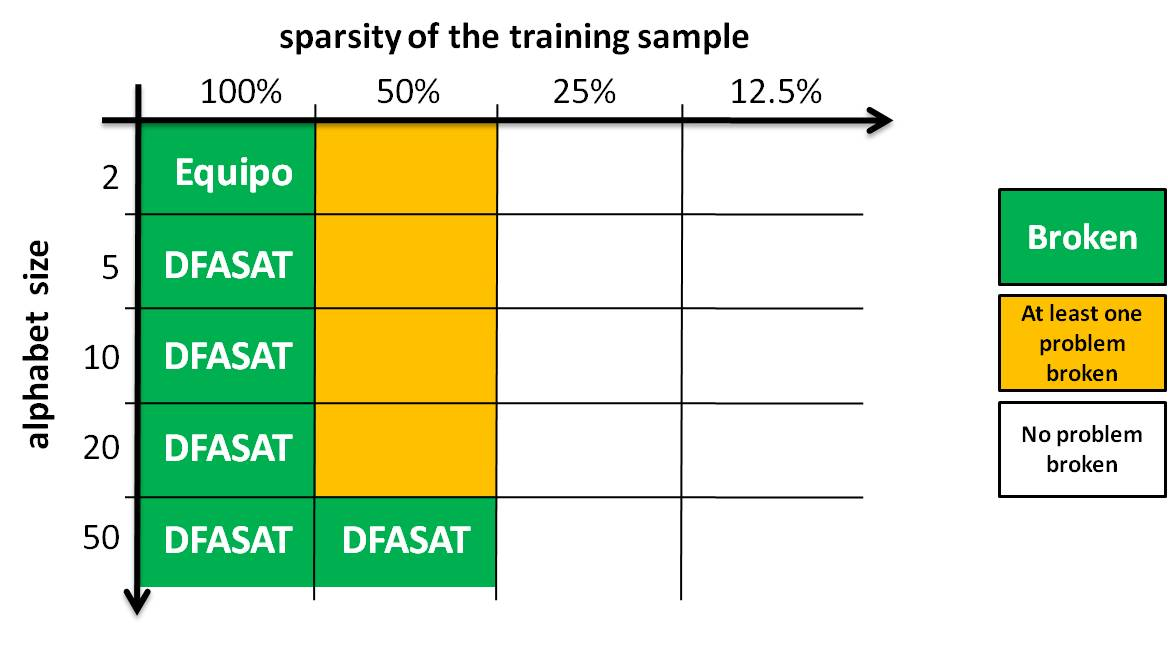
\includegraphics[width=9cm]{images/stamina_broken.jpg}
  \end{center}

\end{frame}